\subsection{Bewertung des Sprints}
In diesem Sprint sind verschiedene Aspekte der Anwendung bearbeitet worden und es sind neue Features dazugekommen. Entsprechend wurde das Pausemenü überarbeitet und ein neues Einstellungsmenü hinzugefügt. Die Trainereinstellungen, welche nun über das Einstellungsmenü zu erreichen sind, wurden ebenfalls überarbeitet. Neu hinzugekommen sind hier ein Audioeinstellungspopup und der Button für die Tastatureinstellung. Ebenso wurden die Minimap und das Rendern und Animieren der Sprites überarbeitet. Die Minimap zeigt nun alle Anforderungen der zweiten Veröffentlichung an. Neu implementiert wurde das Dialogsystem inklusive Interaktionen mit NPCs wie zum Beispiel das Auswählen eines Startmonsters und das Heilen der eigenen Monster. Darüber hinaus wurden die Bonusfeatures Musik in der Anwendung und das Handyfeature, welches Hilfestellungen im Spiel bietet, neu implementiert. Zum Schluss wurde begonnen, den Kampfbildschirm zu implementieren.\\
\begin{figure}[H]
    \center
    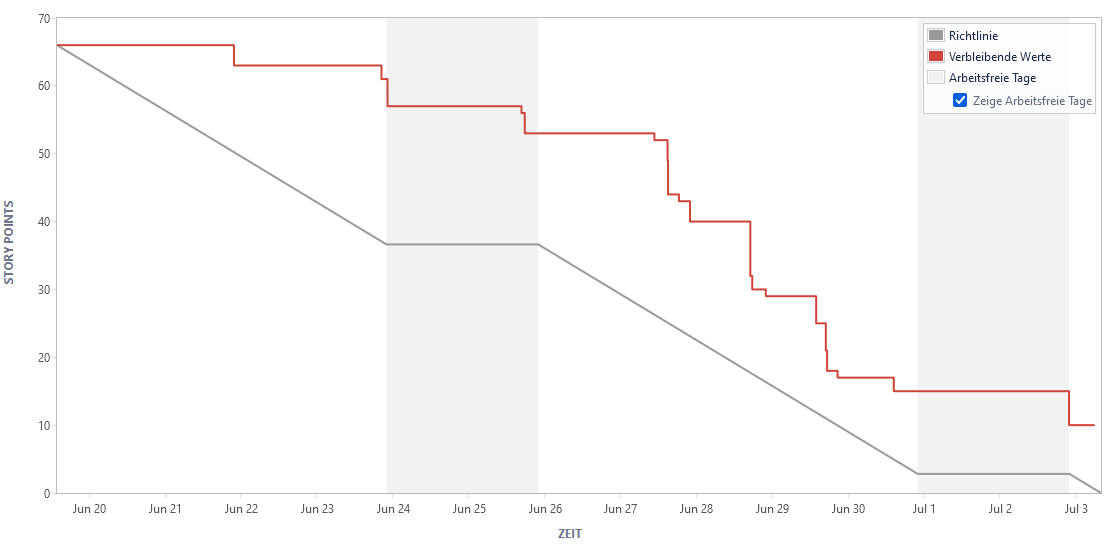
\includegraphics[height=0.5\textwidth]{images/burndown/sprint1Story.png}
    \caption{Burndown-Diagramm: Release 3: Sprint 1 Story Points}
    \label{fig: sprint1Story}
\end{figure}

Wie in Abbildung \ref{fig: sprint1Story} zu sehen ist, wurden nicht alle Storys abgeschlossen. Dies hat zwei Hauptursachen. Demnach wurden zu Beginn des Sprints nicht sehr viele Storys abgearbeitet. Dies wurde zwar versucht in der zweiten Woche wieder aufzuholen, was jedoch nicht komplett gelungen ist. Des Weiteren waren die Storys \hyperlink{S234}{STP23M-234} und \hyperlink{S235}{STP23M-235} von der Story \hyperlink{S224}{STP23M-224} geblockt, welche erst kurz vor Sprintende beendet wurden. Die Story \hyperlink{S271}{STP23M-271}, welche ebenfalls nicht abgeschlossen wurde, kann dabei erst implementiert werden, wenn ein Kampf beendet werden kann, da die Story davon abhängt. \\ Abschließend ist festzuhalten, dass der Sprint zufriedenstellend abgeschlossen wurde, auch wenn nicht alle Storys optimal ausgewählt worden sind.

\subsubsection{Erhöhung der Vorgänge}
Im ersten Sprint der dritten Veröffentlichung gab es eine Umfangsänderung.
\begin{figure}[H]
    \center
    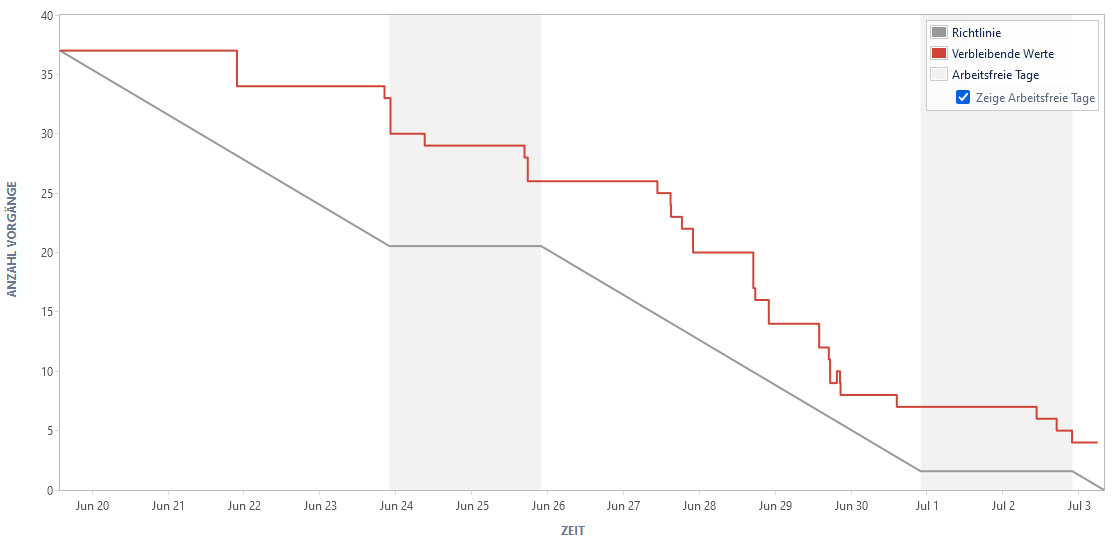
\includegraphics[height=0.5\textwidth]{images/burndown/sprint1vorg.png}
    \caption{Burndown-Diagramm: Release 3: Sprint 1 Vorgänge}
    \label{fig: sprint1vorg}
\end{figure}
Gegen Ende des Sprints am 19.06. wurde der Bug \hyperlink{S433}{STP23M-433} hinzugefügt. Dieser Vorgang ist allerdings schnell abgearbeitet worden und hatte keinen großen Einfluss auf den Sprint.

\subsubsection{Zeitschätzung}
Für alle Vorgänge des ersten Sprints gab es eine Zeitschätzung von insgesamt 90 Stunden und 15 Minuten. Tatsächlich benötigt wurden 105 Stunden und 33 Minuten. Dies ist eine Abweichung von circa 15 Stunden. Die Storys haben dabei allerdings weniger Zeit benötigt als geschätzt und die Aufgaben und Bugs mehr als geschätzt. Diese hohe Diskrepanz ist vor allem mit der Aufgabe \hyperlink{S418}{STP23M-418} zu erklären, welche 16 Stunden länger gedauert hat. 